\documentclass{beamer}

\usetheme{CambridgeUS}

\usepackage{enumerate}
\usepackage{float}
\usepackage{graphicx}
\usepackage{color}
\usepackage{url}
\usepackage{ulem}

\newcommand{\red}[1]{\textcolor{red}{#1}}
\newcommand{\blue}[1]{\textcolor{blue}{#1}}

\title{CS100 Recitation 1}
\author{GKxx}
\date{Februrary 21, 2022}

\begin{document}

\begin{frame}
    \maketitle
\end{frame}

\begin{frame}{Contents}
    \tableofcontents
\end{frame}

\section{C/C++ Environment Setting up}

\subsection{Basic Knowledge}

\begin{frame}{Editors, Compilers and IDEs}
    \begin{itemize}
        \item A \blue{compiler} translates the program written in a high-level language so that the computer can run it.
        \begin{itemize}
            \item \texttt{GCC}, \texttt{Clang}, \texttt{Visual C++} compiler, \dots
        \end{itemize}
        \pause
        \item An \blue{editor} is something where you can edit text.
        \begin{itemize}
            \item \texttt{Notepad}, \texttt{Word}, and even your phone memo.
            \pause
            \item But we need a \text{code editor} which provides more help for coding.
            \item \texttt{Visual Studio Code}, \texttt{Vim}, \texttt{Sublime Text}, \texttt{Notepad++}, \dots
        \end{itemize}
        \pause
        \item IDE: \textbf{I}ntegrated \textbf{D}evelopment \textbf{E}nvironment,
        \begin{itemize}
            \item \(=\) editor \(+\) compilers \(+\) debuggers \(+\cdots\).
            \item \texttt{Visual Studio}, \texttt{Qt}, \texttt{CLion}, \texttt{Dev-C++}, \dots
        \end{itemize}
    \end{itemize}
\end{frame}

\subsection{Installation of Compiler}

\begin{frame}{GCC and MinGW}
    \begin{itemize}
        \item \blue{GCC} is the \textbf{G}NU \textbf{C}ompiler \textbf{C}ollection, an optimizing compiler produced by the \blue{GNU Project} supporting various \blue{programming languages}, \blue{hardware architectures} and \blue{operating systems}.
        \item \blue{MinGW} is short for \textbf{Min}imalist \textbf{G}NU for \textbf{W}indows.
        \pause
        \item For Linux, install GCC directly is ok.
        \item For Windows, you may need MinGW (or, probably MinGW-w64).
    \end{itemize}
\end{frame}

\begin{frame}{MinGW}
    \begin{itemize}
        \item Download the package provided in the Resources page.
        \item Unzip it and place the \texttt{mingw64} folder in the \texttt{C} drive.
        \begin{figure}[h]
            \centering
            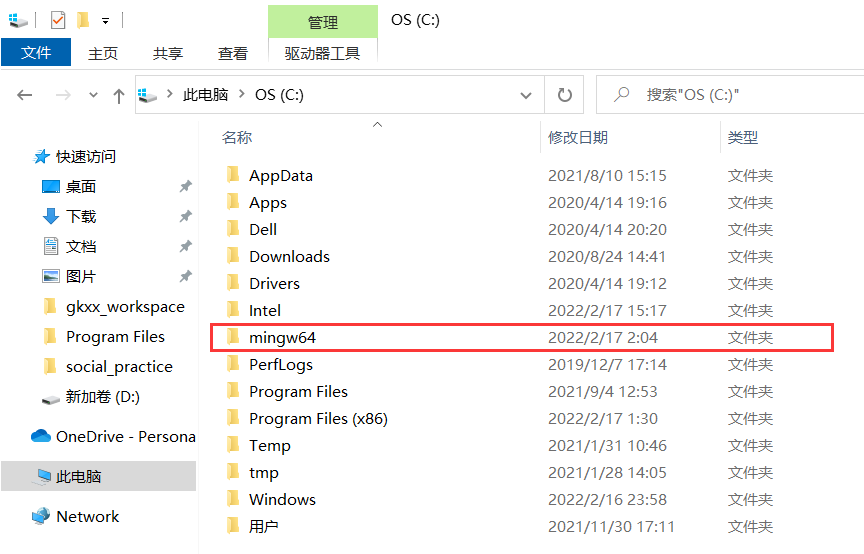
\includegraphics[width=0.8\textwidth]{figures/mingw_in_c.png}
        \end{figure}
    \end{itemize}
\end{frame}

\begin{frame}{MinGW}
    \begin{itemize}
        \item Now the compiler is installed, but it could not be invoked conveniently. We need to add it to the \texttt{Path} \blue{environment variable}.
        \item Press \texttt{Win} and search `env'. Choose `Edit the system environment variables'.
        \begin{figure}[h]
            \centering
            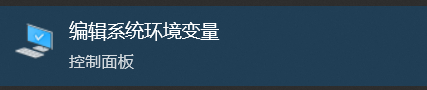
\includegraphics[width=0.5\textwidth]{figures/start_env.png}
        \end{figure}
        \item Click the `Environment variables ...' button.
    \end{itemize}
\end{frame}

\begin{frame}{MinGW}
    \begin{figure}[h]
        \centering
        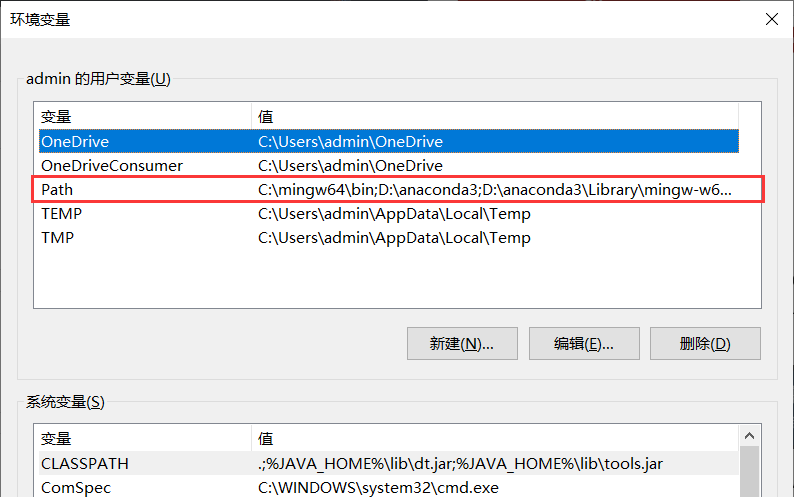
\includegraphics[width=0.8\textwidth]{figures/env_var.png}
    \end{figure}
\end{frame}

\begin{frame}{MinGW}
    \begin{itemize}
        \item Add a new value `\texttt{C:\textbackslash mingw64\textbackslash bin}'.
        \begin{figure}[h]
            \centering
            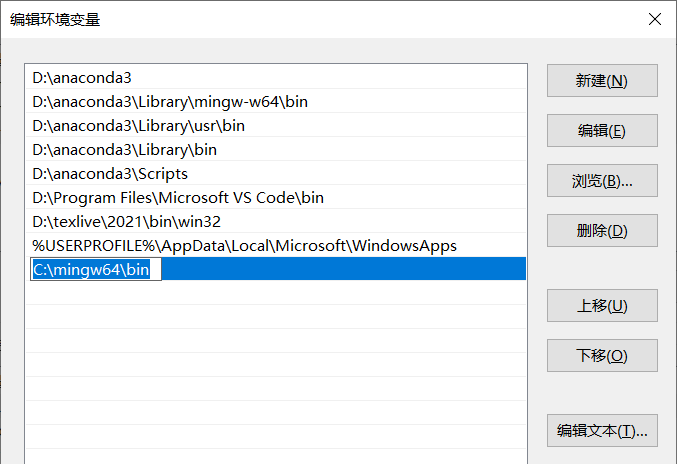
\includegraphics[width=0.8\textwidth]{figures/added.png}
        \end{figure}
    \end{itemize}
\end{frame}

\begin{frame}{MinGW}
    \begin{itemize}
        \item Press \texttt{Win}\(+\)\texttt{r} to open a cmd.
        \item Type `gcc' and press \texttt{Enter}. The following shows that \texttt{gcc} is correctly invoked.
        \begin{figure}[h]
            \centering
            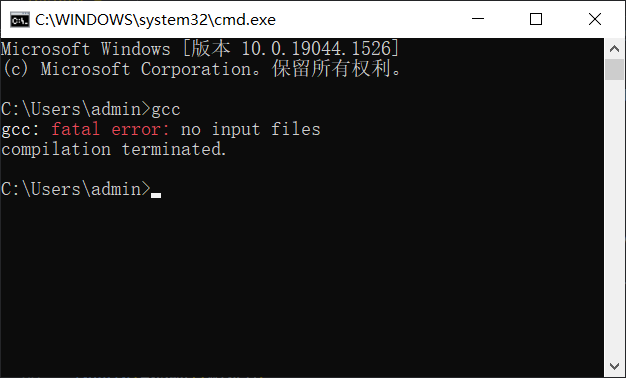
\includegraphics[width=0.8\textwidth]{figures/cmd_gcc.png}
        \end{figure}
    \end{itemize}
\end{frame}

\begin{frame}{MinGW}
    You can use `\texttt{--version}' to see more information about the compilers.
    \begin{figure}[h]
        \centering
        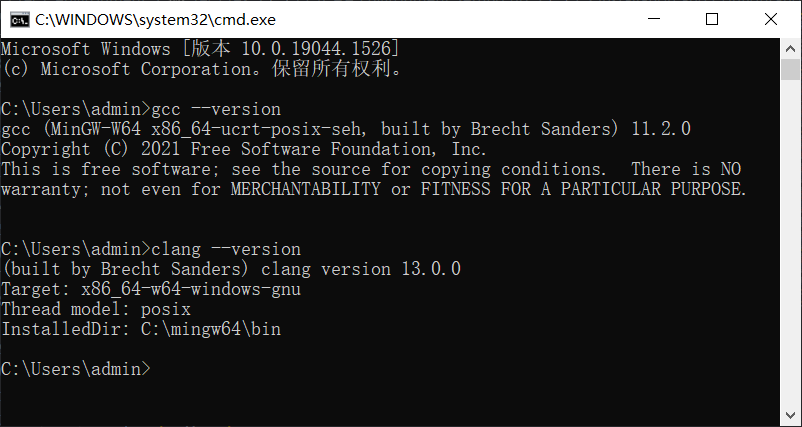
\includegraphics[width=0.8\textwidth]{figures/compiler_versions.png}
    \end{figure}
\end{frame}

\begin{frame}{For Linux (Ubuntu)}
    \begin{itemize}
        \item `\texttt{sudo apt install build-essential}' gets everything done.
        \item If you want compilers of newer versions:\\
        \texttt{sudo add-apt-repository ppa:ubuntu-toolchain-r/test}\\
        \texttt{sudo apt update}\\
        \texttt{sudo apt install gcc-11}
        \item You can search for more on your own.
    \end{itemize}
\end{frame}

\begin{frame}{For Mac OS X}
    \begin{figure}[h]
        \centering
        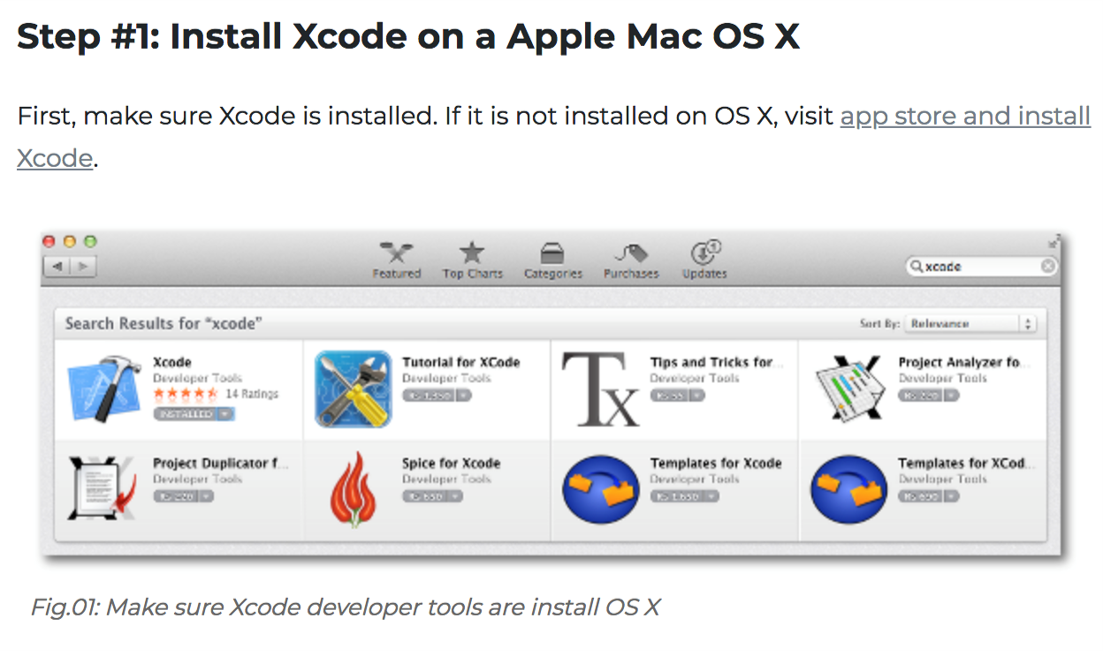
\includegraphics[width=0.9\textwidth]{figures/install_xcode.png}
    \end{figure}
\end{frame}

\begin{frame}{For Mac OS X}
    \begin{figure}[h]
        \centering
        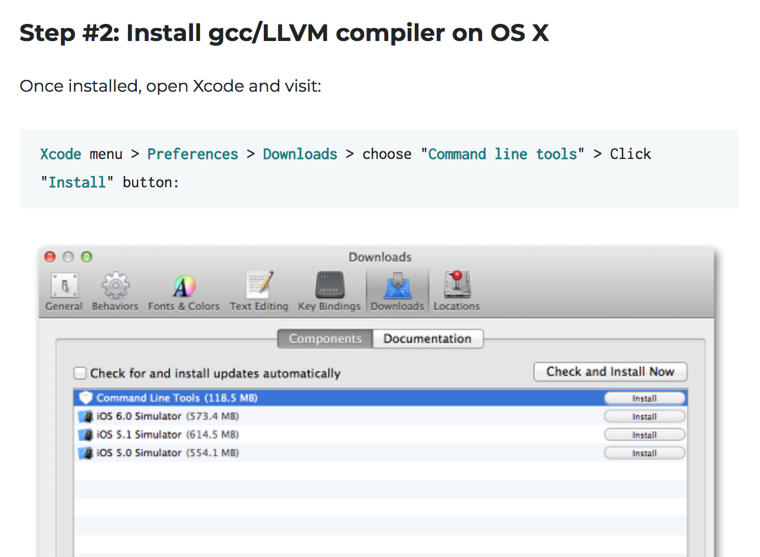
\includegraphics[width=0.8\textwidth]{figures/install_cmd_tools.png}
    \end{figure}
\end{frame}

\begin{frame}{For Mac OS X}
    \begin{figure}[h]
        \centering
        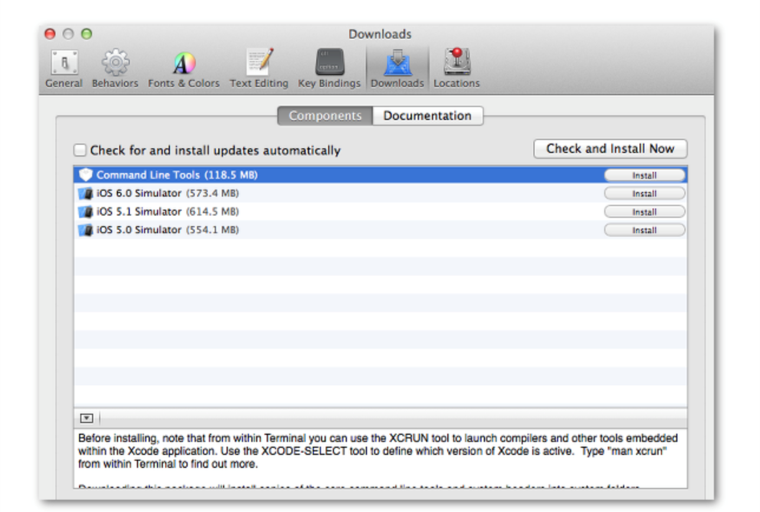
\includegraphics[width=0.9\textwidth]{figures/install_cmd_tools_2.png}
    \end{figure}
\end{frame}

\begin{frame}{For Mac OS X}
    \begin{itemize}
        \item Verify that it is working: `\texttt{gcc --version}'
    \end{itemize}
    \begin{figure}[h]
        \centering
        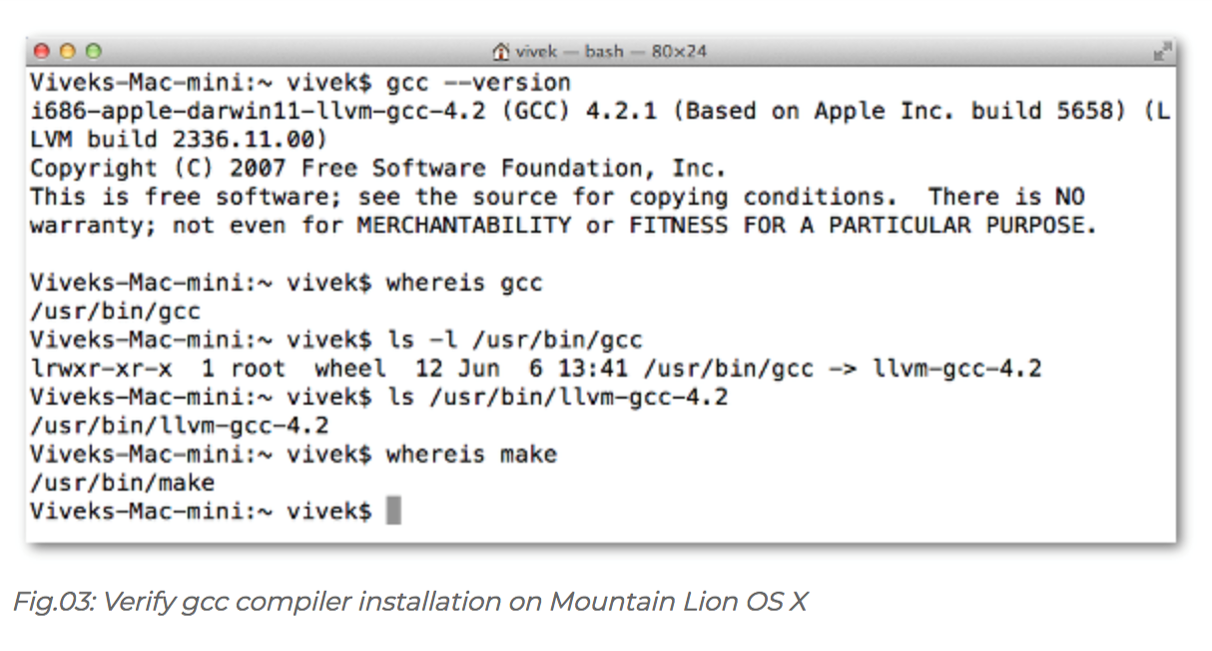
\includegraphics[width=0.9\textwidth]{figures/mac_verify_gcc.png}
    \end{figure}
\end{frame}

\subsection{Installation and Configuration of VSCode}

\begin{frame}{Installation}
    \begin{itemize}
        \item Install \texttt{VSCode} from \url{code.visualstudio.com}.
        \item For Linux users, \textbf{DO NOT} install it via \texttt{snap} or you may encounter trouble.
        \pause
        \item Run the installer. It is recommended to install it in the \texttt{D} or \texttt{E} drive, e.g. \texttt{D:\textbackslash Program Files\textbackslash Microsoft VS Code\textbackslash}.
    \end{itemize}
\end{frame}

\begin{frame}{Extensions}
    Recommended extensions:
    \begin{itemize}
        \item \texttt{Code Runner}, \texttt{C/C++}, \texttt{C/C++ Clang Command Adapter}, \texttt{C++ Intellisense}.
        \item \texttt{Bracket Pair Colorization Toggler}, \texttt{vscode-icons}.
        \item \texttt{One Dark Pro} and \texttt{GitHub Theme}: color themes.
        \item \sout{\texttt{GlassIt-VSC}, \texttt{Cloudmusic}, \texttt{QQ}, \texttt{Zhihu On VSCode}, \dots}
    \end{itemize}
    You may also need \texttt{Chinese (Simplified) Language Pack for Visual Studio Code}.
\end{frame}

\begin{frame}{Configuration}
    \begin{itemize}
        \item Create a folder for CS100, e.g. \texttt{D:\textbackslash CS100}. This will be viewed as a \blue{workspace}.
        \pause
        \item \texttt{VSCode} has `\(n+1\)' configurations, where \(n\) is the number of workspaces and the `\(+1\)' refers to the global (user's) one.
        \item The configuration of each workspace is done by some \texttt{json} files in a special folder \texttt{.vscode}.
        \pause
        \item Remember to always \blue{open \texttt{VSCode} first and then open the workspace}, instead of open a single file directly. Otherwise your configuration for workspace wouldn't work.
    \end{itemize}
\end{frame}

\begin{frame}{Configuration}
    Global settings:
    \begin{figure}[h]
        \centering
        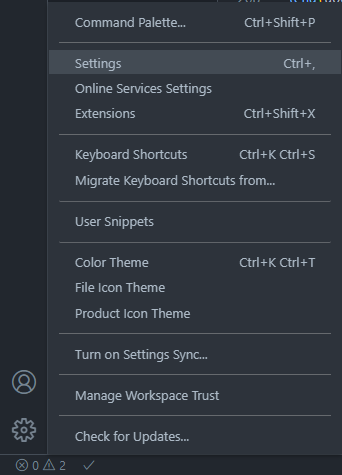
\includegraphics[height=0.75\textheight]{figures/vsc_global.png}
    \end{figure}
\end{frame}

\begin{frame}{Configuration}
    \begin{itemize}
        \item Code-runner: Save File Before Run\quad\blue{true}
        \item Code-runner: Run In Terminal\quad\blue{true}
        \item Code-runner: Ignore Selection\quad\blue{true}
        \item Editor: Format On Type\quad\blue{true}
        \item Editor: Accept Suggestion On Enter\quad\blue{off}
    \end{itemize}
\end{frame}

\begin{frame}{Configuration}
    \begin{itemize}
        \item Create a folder \texttt{D:\textbackslash CS100\textbackslash .vscode} for your workspace configurations.
        \item Create two files \texttt{settings.json} and \texttt{c\_cpp\_properties.json}. Copy the contents from \url{https://www.luogu.com.cn/paste/scc7i5yq}.
        \pause
        \item Create a hello-world program somewhere in this workspace, e.g. \texttt{D:\textbackslash CS100\textbackslash tmp\textbackslash hello.c}.
        \item There will be a `Run Code' button on the top-right corner. Or you can press \texttt{Ctrl+Alt+N} to run the code.
    \end{itemize}
\end{frame}

\begin{frame}{Configuration}
    \begin{itemize}
        \item Pressing this button, the \texttt{Code Runner} extension runs the command we wrote in \texttt{"code-runner.executorMap"} in \texttt{settings.json}.
        \item It is run in the terminal of \texttt{VSCode}, which is the same as in cmd.
        \item The \texttt{Code Runner} extension gets you free from typing the same compilation command manually over and over again. (You may have a try of typing it manually.)
    \end{itemize}
\end{frame}

\begin{frame}{Configuration}
    For the debugging part:
    \begin{itemize}
        \item Print statement debugging is effective, although \texttt{VSCode} says that it is `a thing of the past'.
        \item To use the tools for debugging in \texttt{VSCode}, press \texttt{F5}.
        \item Choose `GDB/LLDB', and then choose `gcc'. If you wish to use the LLVM debuggers, you need to install `lldb-mi' on your own.
        \item Wait a second and the files for debugging are generated automatically. (\texttt{launch.json} and \texttt{tasks.json})
    \end{itemize}
\end{frame}

\section{Foundation of C}

\begin{frame}
    ???
\end{frame}

\end{document}